\section{Evaluation Methodology}\label{sec:methodology}
The evaluation follows two connected questions: what repeated compromise reveals about a protected embedding, and how compact references trade storage against recognition and security. Figure~\ref{fig:methodology} summarizes the workflow. Official pairs assess benchmark verification and renewal, while separate custom protocols assess learned linkage and reconstruction. Identities used for testing are excluded from attack fitting and threshold selection. Payload accounting accompanies the measured outcomes.

Table~\ref{tab:notation} introduces the principal symbols before the mathematical formulation.
% Nonfloating to ensure that notation precedes the equations.
\par\medskip\noindent\begin{minipage}{\columnwidth}
\makeatletter\def\@captype{table}\makeatother
\caption{Notation used in the protection and evaluation models.}
\label{tab:notation}\centering\footnotesize
\renewcommand{\arraystretch}{1.12}
\begin{tabularx}{\columnwidth}{@{}p{1.65cm}>{\raggedright\arraybackslash}X@{}}
\toprule Symbol & Meaning \\\midrule
$I,f_\theta$ & Aligned face image and frozen feature encoder.\\
$x,z,g$ & Unit raw embedding, unit projection input, and preprocessing map from $x$ to $z$.\\
$d_0,d,m$ & Raw dimension (512), projection-input dimension, and template length in bits.\\
$\unit(u)$ & Vector normalization, $u/\|u\|_2$ for $u\ne0$.\\
$k,q,K$ & Historical key, fresh query key, and number of exposed historical records.\\
$W_k,b_k,y_k$ & Keyed $d\times m$ projection, binary template, and signed template $2b_k-1$.\\
$\mu,U_d$ & Fitted PCA mean and retained eigenvector basis.\\
$D_k,H_d,S_k$ & Sign diagonal, normalized Hadamard matrix, and coordinate selector for SRHT.\\
$s_H,\tau,\alpha$ & Bit-agreement score, acceptance threshold, and validation FAR target.\\
$\mathcal E_K,\mathcal I_K$ & Exposed-key set and information available to the inversion attacker.\\
$v_K,a,c$ & Mean signed backprojection and fitted coordinate scales and offsets.\\
$\hat z,\hat x$ & Reconstructed projection input and raw embedding.\\
$x_a,x_b$ & Exposed source embedding and a different-photo enrollment embedding.\\
$\rho_{\mathcal T}$ & Training-only projected norm used for PCA lifting.\\
$A_K,\mathcal F_K$ & Stacked measurement matrix and closed feasible set of unit directions.\\
$B_m,S_m(N)$ & Bytes per template and payload for $N$ stored references.\\
$\mathcal G,\mathcal J$ & Genuine and impostor score sets.\\
$\hat\theta,\Delta$ & Estimated rate and paired configuration difference.\\
$S,U,w_i^{(b)}$ & Split count, unique identity count, and identity multiplicity in bootstrap draw $b$.\\
\bottomrule
\end{tabularx}
\tabnote{TAR, FAR, and ASR denote genuine, impostor, and attack acceptance rates. Dimensions distinguish vectors from scalars; subscripts identify keys, coordinates, or evaluation conditions.}
\end{minipage}\par\medskip

\begin{figure}[!t]
\centering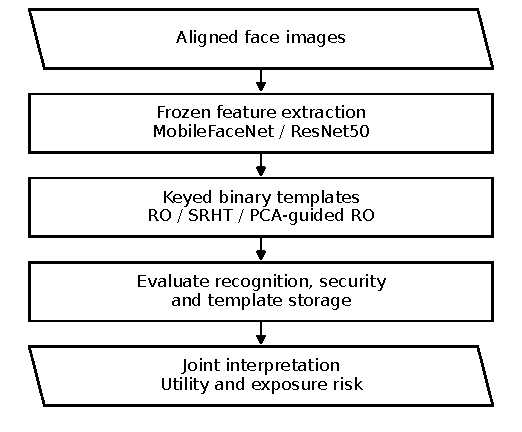
\includegraphics[width=\columnwidth]{methodology.pdf}
\caption{Overview of the evaluation: matched feature extraction and keyed protection feed recognition, security, and template-storage analyses.}
\label{fig:methodology}
\fignote{The workflow links repeated-exposure security with template-storage accounting; device performance is outside the measured scope.}
\end{figure}


Let $I$ denote an aligned facial image, $f_\theta$ a frozen encoder, $d_0=512$ the raw feature dimension, $d$ the projection-input dimension, and $m$ the protected length. The normalized feature and protected representation are
\begin{equation}
 x=\frac{f_\theta(I)}{\|f_\theta(I)\|_2},\qquad z=g(x)\in\mathbb S^{d-1},
\end{equation}
where $\mathbb S^{d-1}$ is the unit sphere. The operator $\unit(u)=u/\|u\|_2$ applies to nonzero vectors. Indices $k$ and $q$ identify historical and fresh keys, respectively; $K$ counts exposed historical records, not identities. In the inversion experiment, all $K$ records encode the same source photograph. A second photograph of the same identity supplies the cross-image enrollment reference. This distinction separates renewal exposure from variation across capture sessions.



For either encoder, $g$ is the identity map or a normalized PCA mapping. Applying the keyed matrix $W_k\in\mathbb{R}^{d\times m}$ and retaining its projection signs gives the $m$-bit template:
\begin{equation}
 b_k(x)=\mathbb{I}[W_k^\top g(x)\geq0]\in\{0,1\}^{m}.
\end{equation}
Protected templates are compared by their fraction of agreeing bits:
\begin{equation}
 s_H(b,b')=1-\frac{1}{m}\sum_{j=1}^{m}(b_j\oplus b'_j).
\end{equation}
A protected comparison is accepted when $s_H\geq\tau$; raw embeddings are compared by cosine similarity. TAR measures acceptance among genuine comparisons, FAR among impostor comparisons, and ASR among attack submissions. The validation FAR target controls threshold calibration and must be distinguished from the FAR subsequently observed on test data.


For RO, a seeded Gaussian matrix admits the thin factorization
\begin{equation}
 G_k=Q_kR_k,\quad Q_k^\top Q_k=I_m,\quad W_k=Q_k.
\label{eq:ro}
\end{equation}
The frozen QR sign convention and matrix shape are retained. CFP E06--E07 factorizes a square matrix and selects its first $m$ columns; the original LFW implementation uses reduced QR. These constructions share orthogonality but need not generate the same seeded bits.

For SRHT, let $D_k$ be a diagonal matrix of keyed Rademacher signs, $H_d$ the normalized Hadamard matrix, and $S_k\in\{0,1\}^{d\times m}$ select distinct keyed coordinates. Then
\begin{equation}
 W_k=D_kH_d^\top S_k,\quad
 W_k^\top z=S_k^\top H_dD_kz.
\label{eq:srht}
\end{equation}
Here $H_d^\top H_d=I_d$ and the tested dimensions admit a Hadamard transform. A positive scalar multiplier does not change the sign template. The stored implementation convention, including coordinate ordering, determines the reproducible bits.

PCA-guided RO first estimates a mean $\mu$ and leading eigenvectors from the permitted fitting set $\mathcal C$:
\begin{align}
 \mu&=|\mathcal C|^{-1}\sum_{i\in\mathcal C}x_i,\\
 C&=|\mathcal C|^{-1}\sum_{i\in\mathcal C}(x_i-\mu)(x_i-\mu)^\top,\\
 CU_d&=U_d\Lambda_d,\qquad g(x)=\unit\!\left(U_d^\top(x-\mu)\right).
\label{eq:pca}
\end{align}
No whitening is applied. The dimension is $d=256$ for 128-bit templates and $d=512$ for CFP 512-bit templates. The latter is a full centered rotation rather than dimensionality reduction. Original attack protocols fit PCA on separate calibration identities; the LFW encoder comparison uses the fold-specific exclusions in Section~\ref{sec:setup}.


For $N$ stored references and float32 raw features, template-only storage and its reduction are
\begin{align}
 B_m&=\lceil m/8\rceil,\quad B_{\rm raw}=4d_0=2048,\\
 S_m(N)&=NB_m,\quad R_m=B_{\rm raw}/B_m,\\
 \eta_m&=100\left(1-B_m/B_{\rm raw}\right)\%.
\label{eq:storage}
\end{align}
The tested lengths are byte-aligned. A useful system-level accounting identity is
\begin{equation}
 S_{\rm total}=S_m(N)+S_{\rm models}+S_{\rm operators}
 +S_{\rm keys}+S_{\rm metadata}.
\end{equation}
Only $S_m(N)$ is quantified here. Dense projection requires $O(dm)$ arithmetic operations; a fast Hadamard implementation requires $O(d\log d)$ before coordinate selection. PCA adds a dense $d_0$-to-$d$ mapping, and packed matching needs $O(\lceil m/w\rceil)$ XOR/popcount operations for word width $w$. These are algorithmic operation counts, not measured latency or energy, and they do not establish that the executed implementation achieves the fast-transform bound.

MobileFaceNet and binary Hamming matching were selected with constrained devices in mind. This paper compares their template-storage choices using measured TAR, FAR, linkage, and ASR. The experiments do not measure on-device response time, peak memory, power, or energy. Public kiosks and smart gadgets are motivating deployment examples, not evaluated platforms. This boundary prevents a smaller template from being mistaken for a demonstrated reduction in total system cost.


Table~\ref{tab:threat} separates the attacker assumptions. The linkage attacker receives $K$ older bit strings and a query template under another key. It does not receive projection operators or the target's raw embedding. The inversion attacker also receives the old operators and template/embedding pairs from other training identities. The algorithm and public PCA model are known. The fresh query operator is hidden during reconstruction and applied only by the verifier.

\begin{table*}[t]
\caption{Attacker access and the security question tested.}
\label{tab:threat}\centering\small
\begin{tabularx}{\textwidth}{@{}>{\raggedright\arraybackslash}p{2.3cm}>{\raggedright\arraybackslash}p{4.5cm}>{\raggedright\arraybackslash}X@{}}\toprule
Experiment & Available information or input & Interpretation \\\midrule
Verification utility & Legitimate same-key reference and probe & Recognition at a separately calibrated threshold.\\
Revoked replay & Unchanged old bit string; new-key reference & Accidental acceptance after renewal with metadata bypassed.\\
Template-only linkage & Historical bit strings and fresh query template & Learned same-identity discrimination without operators.\\
Embedding inversion & Old bit strings, old operators, auxiliary training pairs & Digital embedding-input acceptance under an unexposed key.\\
Image/camera attack & Would require image synthesis or sensor presentation & Outside the experiments; no corresponding success claim.\\\bottomrule
\end{tabularx}
\tabnote{Each test uses the stated attacker information; image and camera attacks are outside scope.}
\end{table*}

A system may reject an outdated reference through a version check before evaluating its similarity. To isolate matching behavior, the replay test bypasses that check and submits the old bits unchanged to the renewed matcher. Inversion instead submits an estimated embedding, which the verifier transforms using its fresh key. Success in this latter test presupposes access to a digital embedding-input interface.


With signed bits $y_k=2b_k-1$, the analytical estimate averages backprojections from the exposed keys:
\begin{equation}
 v_K=\frac{1}{K}\sum_{k\in\mathcal{E}_K}W_k y_k,
 \qquad \hat z_{\mathrm{an}}=\unit(v_K).
\end{equation}
The set $\mathcal{E}_K$ contains exposed keys only. A calibrated version fits one scale and one offset per coordinate using training identities:
\begin{equation}
 \hat z_{\mathrm{cal}}=\unit(a\odot v_K+c).
\end{equation}
For coordinate $j$, the fitted values are $a_j=\operatorname{Cov}(v_j,z_j)/\max(\operatorname{Var}(v_j),10^{-8})$ and $c_j=\bar z_j-a_j\bar v_j$. No nonlinear decoder or target-specific fitting is used. A PCA estimate is mapped back through the public basis and mean. The inverse uses a projected magnitude estimated from training data: the mean for CFP and the median for LFW. It does not use the unknown target magnitude.

Let $x_a$ be the exposed photograph and $x_b$ a different enrollment photograph of the same person. The main attack measure is acceptance of the reconstruction against $x_b$ under a fresh key:
\begin{equation}
 \ASR=\frac{1}{N}\sum_{i=1}^{N}\mathbb{I}
 [s_H(b_{q_i}(\hat x_i),b_{q_i}(x_{b,i}))\geq\tau_{q_i}].
\end{equation}
Results average the prescribed identities, trials, and splits. Using another photograph tests whether recovery remains useful beyond the exposed image. Additional measures are acceptance against that exposed image, cosine similarity to its embedding, and acceptance by the raw cosine matcher at its own threshold. Uninformed submissions use the normalized mean training embedding in LFW and embeddings of non-target training identities in CFP. These controls are distinct from the impostor comparisons used to estimate FAR.



Stacking the compromised operators yields
\begin{equation}
 A_K=\begin{bmatrix}W_{k_1}^\top\\\vdots\\W_{k_K}^\top\end{bmatrix},
 \quad y_K=\begin{bmatrix}y_{k_1}\\\vdots\\y_{k_K}\end{bmatrix},
 \quad y_K=\operatorname{sign}(A_Kz).
\end{equation}
Each nonzero signed measurement restricts $z$ to a hemisphere. A closed relaxation of the consistent directions is
\begin{equation}
 \mathcal F_K=\{u\in\mathbb S^{d-1}:\operatorname{diag}(y_K)A_Ku\succeq0\}.
\label{eq:feasible}
\end{equation}
Negative bits use a strict inequality under the implementation's zero-tie convention; the closed set includes its boundary. With the nested exposure schedule, $\mathcal F_{K+1}\subseteq\mathcal F_K$. Additional signs cannot enlarge this feasible set, although redundant measurements need not shrink it. This geometric observation does not guarantee monotone acceptance for a finite-data reconstruction algorithm.

For an idealized independent Gaussian row $a\sim\mathcal N(0,I_d)$ and fixed unit $z$,
\begin{equation}
 \mathbb E[a\,\operatorname{sign}(a^\top z)]=\sqrt{2/\pi}\,z.
\label{eq:gaussian}
\end{equation}
To see this, write $a=tz+a_\perp$, where $t\sim\mathcal N(0,1)$ and $a_\perp$ is independent with zero mean. The expectation becomes $\mathbb E|t|z$. This identity motivates signed backprojection and is consistent with one-bit recovery theory~\cite{plan2013,jacques2013}. The experiment uses correlated orthogonal or structured rows and non-Gaussian face features; therefore, this illustration is not a recovery theorem for RO, SRHT, or PCA-guided RO. Likewise, $Km$ is a count of binary observations, not an estimate of independent information bits or cryptographic security strength.


Coordinate calibration uses ordinary least-squares slopes and intercepts estimated from auxiliary training examples. Ignoring the numerical variance floor, the fit for coordinate $j$ minimizes
\begin{equation}
 \min_{a_j,c_j}\sum_{i\in\mathcal T}
 \left[z_{ij}-(a_jv_{K,ij}+c_j)\right]^2.
\end{equation}
The $10^{-8}$ floor stabilizes nearly constant coordinates and is not a tuned ridge penalty. For PCA protection, lifting back to the raw feature space uses
\begin{equation}
 \hat x=\unit(\mu+\rho_{\mathcal T}U_d\hat z),
\label{eq:lift}
\end{equation}
where $\rho_{\mathcal T}$ is the training-only mean projected norm in CFP and median projected norm in LFW. For RO and SRHT, $\hat x=\hat z$. Source reconstruction quality is $c_{\rm src}=\hat x^\top x_a$; cross-image quality is $c_{\rm cross}=\hat x^\top x_b$. Neither quantity determines acceptance without the fresh transformation and threshold.

The attack's information set is $\mathcal I_K=\{(b_k(x_a),W_k):k\in\mathcal E_K\}$ plus the public preprocessing and auxiliary training information. Reconstruction has the form $\hat x=\mathcal A(\mathcal I_K)$, with $q\notin\mathcal E_K$. The verifier alone computes $b_q(\hat x)$ and compares it with $b_q(x_b)$. Thus, concealing the fresh operator is an explicit experimental constraint; it does not erase constraints already disclosed by the historical operators.


For genuine scores $\mathcal G$ and impostor scores $\mathcal J$, the empirical rates at threshold $\tau$ are
\begin{align}
 \widehat{\TAR}(\tau)&=|\mathcal G|^{-1}\sum_{s\in\mathcal G}\mathbb I[s\geq\tau],\\
 \widehat{\FAR}(\tau)&=|\mathcal J|^{-1}\sum_{s\in\mathcal J}\mathbb I[s\geq\tau].
\end{align}
Protected scores lie on the grid $\{0,1/m,\ldots,1\}$. The frozen validation rule selects the least restrictive attainable acceptance set containing at most $\lfloor\alpha|\mathcal J_{\rm val}|\rfloor$ impostor scores. A threshold just above a tied boundary excludes the entire tied group. Consequently, calibration at target $\alpha$ need not achieve equality, and observed test FAR is a separate quantity.

For an old-to-new key transition, unchanged-template replay is
\begin{equation}
 \widehat R_{k\to q}=\frac1n\sum_{i=1}^n
 \mathbb I[s_H(b_k(x_{a,i}),b_q(x_{b,i}))\geq\tau_q].
\end{equation}
This definition follows the image pairing prescribed by the replay protocol; it differs from fresh-key ASR because no reconstruction is submitted. For learned linkage score $\ell$, ROC AUC estimates
\begin{equation}
 \Pr(\ell_{\rm same}>\ell_{\rm different})+
 \tfrac12\Pr(\ell_{\rm same}=\ell_{\rm different}).
\end{equation}
AUC is score-specific. Direction-aware basic diagnostics use $\max(\mathrm{AUC},1-\mathrm{AUC})$; learned linkage retains the trained score direction. Neither chance-level AUC nor a low replay rate establishes irreversibility.
